\chapter{Antecedentes}
\label{chap:antecedentes}

En este capítulo se discutirán algunos de los conceptos que se han empleado para la elaboración de este proyecto. En concreto, se hablará sobre los sistemas de recomendación, explicando en que consisten y profundizando especialmente en los sistemas de recomendación híbridos. 

\section{Sistemas de recomendación}
En la vida diaria, las personas recurren a las recomendaciones o críticas por parte de otras cuando sus experiencias personales o conocimientos sobre el tema son insuficientes.  Los sistemas de recomendación actuales desempeñan un papel similar a este proceso. En 1997 Resnick y Varian \cite{Resnick:1997:RS:245108.245121} definieron por primera vez los sistemas de recomendación como sistemas en los que ``la gente proporciona recomendaciones como entrada al sistema, el cual luego se encarga de agregar y redirigir estas a los destinatarios adecuados''. %no se si tengo que citar entre comillas cuando hago mi traducción no oficial
Posteriormente, se ha ampliado esta definición \cite{Burke}, considerando sistemas de recomendación aquellos que generan recomendaciones personalizadas o que son capaces de guiar al usuario hacia elementos que sean de su interés dentro de un amplio abanico de posibilidades. Es esta característica de individualización o recomendación personalizada lo que distingue a estos sistemas de otros como los buscadores simples y los sistemas de recuperación de información.

Estos sistemas son claves hoy en día, donde toda la información que se encuentra en la red en prácticamente cualquier portal trasciende la capacidad de los usuarios para buscar y seleccionar de entre todos los elementos por sí mismo. Un ejemplo de sistema de recomendación es el sistema de la compañía Netflix, que proporciona recomendaciones de películas en base a las anteriores visualizaciones de los usuarios. Esta compañía realizó en 2006 una competición en la que retó a la comunidad, a desarrollar un sistema de recomendación que fuese capaz de derrotar al de la compañía \textit{Cinematch} \cite{Bennett:2007}. Para ello, ofreció al público una pequeña fracción de sus datos en la que se encontraban valoraciones anónimas de usuarios sobre películas. Se inscribieron 20.000 equipos, de los cuales 2.000 presentaron al menos una solución. En 2009 se concedió un premio de 1.000.000 de dolares a un equipo que mejoró la precisión de Cinematch en un 10\%. Todos estos números pueden servir para hacerse una idea del potencial que ofrecen los sistemas de recomendación hoy en día.

\subsection{Evolución histórica de los sistemas de recomendación}

%Se puede añadir los campos existentes previos de los que parte este área de investigación
El primer sistema de recomendación que se desarrollo fue Tapestry \cite{Goldberg:1992:UCF:138859.138867} a comienzos de los 90, y sus desarrolladores lo denominaron con el término \textit{Filtro colaborativo}, el cual fue adoptado por otros desarrolladores, pero que en la actualidad ha quedado en desuso debido principalmente a que los actuales sistemas no solo filtran aquellos elementos o productos que no son deseables, sino que tratan de sugerir aquellos que puedan aportar mayor valor, además de que como se verá más adelante, algunos de los tipos de sistemas de recomendación que fueron apareciendo posteriormente, no tenía en cuenta las opiniones de otros usuarios, pudiendo, por tanto, no ser colaborativos. Este primer sistema pionero, tenía como propósito el de filtrar el correo electrónico,  así como artículos de noticias online. Es especialmente en este campo del filtrado de noticias donde los primeros sistemas de recomendación tuvieron mayor auge. 

 Pese a que este sistema es el primero considerado de recomendación, algunos años antes ya se propusieron trabajos y teorías sobre sistemas para el filtrado de elementos, como el trabajo de Housman y Kaskela \cite{4322444} que buscaba mantener a los científicos informados de los nuevos documentos mediante un matching entre las palabras clave que estos establecían de su interés, y el contenido de los nuevos artículos. Sin embargo, esta estrategia no logró los resultados deseados. Otra aproximación fue la de la creación de modelos de usuario que aparece en el trabajo de Allen \cite{allen1990user}. Por otra parte, el sistema \textit{The information Lens} \cite{Malone:1986:ILI:22339.22340} planteó un enfoque diferente hacia los sistemas de recomendación, estableciendo reglas que se apoyaban en la estructura que tienen la mayoría de los mensajes de correo electrónico y en palabras clave de estos, permitiendo a los usuarios utilizar estas estructuras como plantillas de manera que fuese más fácil para estos establecer los mecanismos de filtro. Todos estos sistemas fueron dando forma a los diferentes tipos y categorías de sistemas de recomendación que existen hoy en día.

\subsection{Clasificación de los sistemas de recomendación}

Desde su aparición, se han realizado distintas clasificaciones de los sistemas de recomendación. En este caso se va a mostrar la clasificación que realizaron Resnick y Varian \cite{Resnick:1997:RS:245108.245121}. De este modo, se establecen una serie de características según las cuales se podría realizar la clasificación de estos sistemas. 

En primer lugar se establecen las siguientes características técnicas:

\begin{itemize}
\item El contenido de la recomendación, es decir, la valoración a los distintos elementos a recomendar. Esta valoración puede ser tan simple como un valor binario (recomendado o no) o algo más complejo como un un porcentaje o un texto.
\item El modo en el que se realizan o recogen las recomendaciones. Las recomendaciones pueden ser realizadas de manera explícita, pero también pueden ser recogidas de manera implícita por el sistema, por ejemplo, analizando las preferencias de los usuarios, las búsquedas y visitas de estos a diferentes portales o las compras previas de estos. Existen mecanismos muy útiles para poder recoger estas recomendaciones implícitas como las cookies en los sistemas web.
\item La identidad de los recomendadores. Esta puede ser la identidad real, un pseudónimo o bien una identidad anónima. Como se verá más adelante, los usuarios prefieren conservar su privacidad en numerosas ocasiones, y pueden ser reacios a compartir información de carácter sensible aun cuando esta información puede ser crucial para el sistema de recomendación, por esta razón es necesario ofrecer mecanismos que les permitan conservar dicha privacidad.
\item Las técnicas de recomendación, es decir, la manera en la que se relacionan las recomendaciones con aquellos que buscan recomendación. Esta es una de las características que permiten mayor flexibilidad en este tipo de sistemas y será analizada en profundidad más adelante.
\item La finalidad de las evaluaciones. Uno de los usos es el de descartar o sugerir elementos. Otra finalidad puede ser la de ordenar los elementos recomendados según un peso, o mostrar para cada elemento el nivel de recomendación. 
\end{itemize}

Además de las características técnicas, otro de los elementos que caracterizan un sistema de recomendación es su dominio, es decir, los elementos o ítems que se recomiendan, y el público que realiza o recibe las distintas recomendaciones.

En lo referente a los elementos sobre los que se aplican las recomendaciones es importante, en primer lugar, definir el tipo de los elementos que se están recomendando. En el Cuadro \ref{tab:items-recommended} se muestran algunos ejemplos de sitios y los elementos que recomiendan. Otro factor importante es el volumen de los elementos que se recomiendan, así como la frecuencia con la que se generan y desaparecen. Es necesario conocer y tener en cuenta estos parámetros ya que se deben de tratar de manera muy distinta unos elementos que se generan con gran frecuencia y tienen un tiempo de vida corto, como pueden ser las noticias de un medio electrónico, en el que es muy importante poder recomendar dichas noticias en un tiempo acotado, a la necesidad de recomendar por ejemplo películas o libros. Es aquí donde asumen gran importancia las técnicas de recomendación. 

Por otro lado, se encuentran los costes que implican el proceso de recomendación y los resultados. Es posible, que el coste de fallar en la recomendación como por ejemplo al no recomendar un buen ítem, sea más alto que el coste de recomendar un ítem incorrecto o viceversa. También es muy relevante el tiempo que conlleva realizar una recomendación. Pueden existir sistemas de recomendación que deban realizar la recomendación en un tiempo crítico, y por tanto, el coste de un análisis intensivo sea mayor que el de obviar buenos ítems o recomendar algunos que no sean los adecuados. Este factor, es altamente dependiente de la configuración de los características técnicas mencionadas anteriormente.  

\begin{table}[hp]
  \centering
  {\small
  


\begin{tabular}{p{.3\textwidth}p{.3\textwidth}}
  \tabheadformat
  \tabhead{Sitio}   &
  \tabhead{Elementos recomendado}\\
\hline
Amazon  & Libros/otros productos \\
\hline
Facebook & Amigos\\
\hline
WeFollow  & Amigos \\
\hline
MovieLnes  & Películas\\
\hline
Nanocrowd  & Películas \\
\hline
Jinni  & Películas\\
\hline
Findory  &  Noticias\\
\hline
Digg  &  Noticias\\
\hline
Zite  &  Noticias\\
\hline
Meehive  &  Noticias\\
\hline
Netflix  & DVDs\\
\hline
CDNOW  &  CDs/DVDs\\
\hline
eHarmony  & Citas\\
\hline
Chemistry  &  Citas\\
\hline
True.com  & Citas\\
\hline
Perfectmatch  &  Citas\\
\hline
CareerBuilder  & Trabajos\\
\hline
Monster  &  Trabajos\\
\hline
Pandora  & Música\\
\hline
Muffin  & Música \\
\hline
StumbleUpon  & Páginas Web\\
\hline
\end{tabular}


% Local variables:
%   coding: utf-8
%   ispell-local-dictionary: "castellano8"
%   TeX-master: "main.tex"
% End:

  }
  \caption[Sitios web y elementos que recomiendan]
  {Sitios web y elementos que recomiendan
    (\textsc{RESNICK}~\cite{Lu})}
  \label{tab:items-recommended}
\end{table}


En el caso de los usuarios involucrados en el proceso de las recomendaciones, tanto aquellos que las realizan como los que las consumen, es necesario conocer los perfiles de estos. Por ejemplo, se debe saber si los usuarios tienden a realizar recomendaciones de numerosos elementos similares, o por el contrario, evalúan solo elementos muy específicos dando lugar a diferentes conjuntos de recomendaciones. También es importante conocer la cantidad de usuarios que componen o compondrían el sistema, y la variedad respecto a los gustos de los usuarios. El sistema y las técnicas a aplicar varían de manera muy notable si existe una gran cantidad de usuarios con gustos similares, o por el contrario existen muy pocos usuarios con perfiles muy especializados y concretos.



\subsection{Técnicas de recomendación}
\label{sec:tecnicas-recomendacion}
Como se ha mencionado anteriormente existen varias técnicas de recomendación que permiten adaptarse a la situación en cuestión. Algunos autores prefieren realizar una clasificación sobre estas técnicas de recomendación más acotada que la que se va a utilizar en este documento\cite{Balabanovic:1997:FCC:245108.245124}, diferenciando entre tres grandes grupos de sistemas de recomendación. Por un lado, distinguen principalmente si son sistemas en los que influyen las valoraciones u opiniones de otros usuarios, a los que se consideran sistemas colaborativos. Si por el contrario lo único que afecta a la recomendación es la valoración previa del usuario sobre los elementos que se recomiendan y las relaciones entre estos elementos, el sistema se considera basado en contenido. Además, si son sistemas que combinan estrategias de los dos anteriores, estos se consideran híbridos. Si bien esta es una clasificación perfectamente válida, y abarca las técnicas más importantes y utilizadas, en este documento se han querido nombrar también otras técnicas utilizadas.


A la hora de elegir una de estas técnicas, es necesario tener en cuenta principalmente tres factores. Por un lado, se encuentran los datos y la información de la que disponemos antes de comenzar el proceso de recomendación, como pueden ser las valoraciones de ciertos usuarios de los ítems, o información sobre dichos ítems. Por otro lado, está la entrada que realiza el usuario, es decir, la información que este comunica al sistema con el propósito de obtener una recomendación. Finalmente, es necesario disponer mecanismo o algoritmo que sea capaz de combinar los dos elementos anteriores para poder llevar a cabo la recomendación. Mediante estos tres factores, se pueden definir un total de cinco técnicas de recomendación. Considerando \textbf{U} como el conjunto de los usuarios de los que se conocen las preferencias, \textbf{I} el conjunto de los ítems sobre los que existen valoraciones, \textbf{u} el usuario para el que realizar la recomendación e \textbf{i} el elemento en cuestión que se está considerando para ser recomendado, en el cuadro \ref{tab:recommendation-techniques} se muestra a grandes rasgos como funcionan estas técnicas en función de los factores anteriores. 


\begin{table}[hp]
  \centering
  {\small
  


\begin{tabular}{p{.15\textwidth}p{.25\textwidth}p{.25\textwidth}p{.25\textwidth}}
  \tabheadformat
  \tabhead{Técnica}   &
  \tabhead{Información previa}      &
  \tabhead{Entrada} &
  \tabhead{Algoritmo}  \\
\hline
Colaborativo & Evaluaciones de \textbf{U} de los elementos en \textbf{I}. & Evaluación de \textbf{u} de los elementos en \textbf{I}. & Identifica a los usuarios en \textbf{U} con perfiles similares a \textbf{u}, y extrapola sus valoraciones de \textbf{i}.\\
\hline
Basada en contenido  & Características de los elementos en \textbf{I}. & Las valoraciones de \textbf{u} de los elementos en \textbf{I}. & Generar un clasificador que adapte el comportamiento respecto a las valoracioes de \textbf{u} y lo use en \textbf{i}. \\
\hline
Demográfica & Información demográfica sobre \textbf{U} y sus evaluaciones de los elementos en \textbf{I}. & Información demográfica sobre \textbf{u}. & Identificar aquellos usuarios que son demográficamente similares a \textbf{u} y extrapolar sus evaluaciones de \textbf{i}. \\
\hline
Basada en utilidad & Características de los elementos en \textbf{I}. & Una función de utilidad sobre los elementos en \textbf{I} que describa las preferencias de \textbf{u}. & Aplicar la función sobre los elementos y determinar la clasificación de \textbf{i}. \\
\hline
Basada en conocimiento & Características de los elementos en \textbf{I}. Conocimiento de como estos elementos cumplen las necesidades del usuario. & Una descripción de las necesidades o intereses de \textbf{u} & Inferir la afinidad del item \textbf{i} con las necesidades de \textbf{u}.\\
\hline
\end{tabular}


% Local variables:
%   coding: utf-8
%   ispell-local-dictionary: "castellano8"
%   TeX-master: "main.tex"
% End:

  }
  \caption[Técnicas de recomendación]
  {Técnicas de recomendación
    (\textsc{BURKE}~\cite{Burke})}
  \label{tab:recommendation-techniques}
\end{table}

A continuación se muestran en más detalle las diferentes técnicas.

%TODO Añadir personality based systems
\subsubsection{Colaborativa}
La técnica colaborativa es probablemente la más usada dentro de este tipo de sistemas. En los sistemas que usan dicha técnica, cada usuario tiene un perfil en el que se encuentran las evaluaciones que ha realizado este de cada elemento. El funcionamiento de esta técnica, consistiría en comparar al usuario, o en este caso su perfil, con el de otros  usuarios a los que se puede considerar sus vecinos, para encontrar las similitudes entre ellos. Usando estas similitudes, se puede extrapolar la información sobre las evaluaciones u opiniones de estos usuarios sobre el ítem que se pretende evaluar o recomendar. De esta manera, si el ítem en cuestión ha sido positivamente valorado por aquellos usuarios que se consideran vecinos del usuario para el que se quiere realizar la recomendación, este ítem será también recomendado a dicho usuario.

Un ejemplo simple de como sería un perfil de usuario en estos sistemas consiste en una estructura de datos en el que se encuentran los elementos evaluados junto con las valoraciones realizadas por el usuario. Los sistemas que emplean esta técnica están pensados para generar relaciones a largo plazo, ya que por norma general mejoran su funcionamiento conforme aumentan las recomendaciones. Es por esto, que en algunos casos es recomendable establecer mecanismos que sean capaces de modificar estos datos en función del tiempo de manera ajena al usuario. Esto es debido a que el usuario puede haber variado sus gustos u opiniones a lo largo de este tiempo, y las evaluaciones pueden no ser fiables. 

Respecto a los algoritmos y medidas utilizados en este tipo de sistemas de recomendación destacan especialmente dos tipos, por una parte, se encuentran los algoritmos basados en memoria\cite{Yu:2004:PMC:956382.956411}. En este tipo de algoritmos, se tienen en cuenta todas las valoraciones realizadas por un usuario. Debido a esto, este tipo de sistemas presentan problemas de escalabilidad en aquellos escenarios en los que existen gran cantidad de usuarios, gran cantidad de evaluaciones por parte de los usuarios o ambos \cite{lee2001collaborative}. Por otra parte, se encuentran los sistemas basados en modelos, en los que se crean modelos probabilísticos a partir de las valoraciones de los usuarios. Existen numerosas técnicas que han sido empleadas para la generación de estos modelos como redes bayesianas, o técnicas de aprendizaje automático como clústers o redes neuronales.

Jonathan Lee Herlocker, en su tesis\cite{herlocker2000understanding}, realizó un estudio de esta técnica, comparando diferentes algoritmos para evaluar la similitud entre los distintos perfiles de usuarios, así como diferentes métricas para evaluar este tipo de sistemas. Tras analizar las métricas para la evaluación de la precisión de las evaluaciones, este llegó a la conclusión de que todas las métricas propuestas desempeñan una ejecución similar, y propone adoptar como estándar la métrica del error medio absoluto o \ac{MAE}. 

\[MAE = \frac{1}{n}\sum_{i=1}^{n}\left | e_{i} \right |\]

Donde \textit{e} es la diferencia para cada estimación \textit{i} entre el valor estimado y el valor real, y \textit{n} es el total de las estimaciones.


\subsubsection{Basada en contenido}
Esta técnica es una extensión de los estudios en el filtrado de información\cite{Hanani:2001:IFO:598287.598363}. A diferencia de la técnica colaborativa en la que se establecían relaciones entre los usuarios, en esta se establecen relaciones entre los los elementos a recomendar y los elementos que ya han sido valorados por el usuario. Se comparan aquellas características o atributos que se encuentran en los diferentes ítems, estableciendo el grado de similitud entre los valores de estas. Usando esta información, es posible sugerir aquellos elementos que tienen características en común con aquellos que el usuario ha valorado positivamente. 

De esta manera, el perfil de usuario se establece basándose en aquellos elementos que han gustado, o dicho de otra manera que el usuario ha valorado positivamente. Es esta característica de poseer un perfil de usuario en el que se encuentran los gustos o intereses de los usuarios, lo que diferencia este tipo de sistemas de los sistemas de filtrado de información convencionales.

Esta técnica puede ser muy útil en un sistema de recomendación por ejemplo de películas, donde encontramos elementos que comparten las mismas características como el reparto, la temática o la fecha de lanzamiento. Además, debido a su relación con los sistemas de recuperación y filtrado de la información, y al trabajo previo desarrollado en este tipo de sistemas, este tipo de técnica es especialmente útil en aquellos casos en los que los elementos a recomendar son descritos de manera textual, o contienen características textuales \cite{Mooney:2000:CBR:336597.336662}. 

%TODO : Añadir las fórmulas para el cálculo de tf y idf

Una de las \textbf{medidas} más usadas para el cálculo de las relaciones entre los diferentes elementos, y su relación con los perfiles de usuario, es la de la frecuencia de término - frecuencia inversa de documento \acs{Tf-idf}\cite{robertson2004understanding}. Esta es una medida numérica que busca identificar las palabras más relevantes en un documento o texto. Para ello, contrasta el número de veces que aparece una palabra en el texto en cuestión(tf), frente al número de veces que aparece en el conjunto de todos los textos (idf). Así pues, si una palabra aparece frecuentemente en un texto pero no así en el conjunto de estos, se dice que esa palabra es representativa de ese texto en concreto. 

Esta técnica suele ser combinada con un sistema vectorial\cite{Salton:1975:VSM:361219.361220} en el que se representan para cada elemento las palabras o características más relevantes junto con su relevancia o peso. Se construyen así los perfiles para cada elemento de los que se pueden recomendar. De la misma manera, es necesario establecer aquellos términos o características que al usuario le parecen interesantes, haciendo una ponderación de los distintos ítems que este ha valorado positivamente, y de los conceptos relevantes que aparecen en estos. Finalmente, se utiliza alguna heurística de puntuación para establecer la relación que existe entre los elementos a recomendar y los perfiles de usuario, o dicho de otra manera, la probabilidad de que ese elemento satisfaga las necesidades o los deseos del usuario. Esta heurística deberá tratar generalmente con vectores.

Otras medidas también usadas en este tipo de sistemas de recomendación son las técnicas de aprendizaje automático\cite{lang1995newsweeder}. Estas técnicas, a diferencia de las anteriores que están basadas en los estudios de la recuperación de información, usan modelos aprendidos de los datos mediante técnicas de aprendizaje en lugar de heurísticas, para calcular los elementos a recomendar. También se pueden utilizar clasificadores bayesianos para estas recomendaciones\cite{Pazzani:1997:LRU:261092.261098}.


\subsubsection{Demográfica}
En este tipo de recomendadores, es necesario establecer una serie de perfiles o clases definidos de manera previa. Posteriormente, se obtiene la información personal de los usuarios y se usa esta para categorizarlos en alguna de las clases demográficas definidas anteriormente. Los mecanismos para obtener estos datos pueden ser variados, usando mecanismos para obtenerlos de manera explícita como puede ser un test, u otros mecanismos que extraigan esta información de manera implícita. Esta técnica es similar a la colaborativa en el uso de los perfiles de los usuarios para sus recomendaciones, sin embargo la ventaja de esta sobre la anterior es que no necesita evaluaciones previas de los ítems por parte de los usuarios.



\subsubsection{Basada en utilidad}
Los sistemas que emplean esta técnica realizan recomendaciones a partir de un cálculo sobre la utilidad que tiene cada elemento para satisfacer las necesidades del usuario. Es necesario por tanto, establecer una función de utilidad para cada usuario, siendo esta función la que componga su perfil. Este tipo de técnica presenta la ventaja de poder incluir en sus cálculos y recomendaciones atributos que no son propios del elemento que se quiere recomendar como tal, como puede ser por ejemplo, la confianza en el vendedor de dicho producto en casos de comercio en línea, o el tiempo de entrega. Esto permite que estos sistemas sean capaces de valorar y negociar de acuerdo a distintas características, por ejemplo negociando el precio en función del tiempo de entrega.

\subsubsection{Basada en conocimiento}
Esta técnica realiza las recomendaciones a parir del conocimiento de como un determinado ítem satisface las necesidades o deseos de un usuario. El perfil de usuario en este tipo de recomendadores será cualquier estructura que sea capaz de representar las necesidades de los usuarios. Del mismo modo, el conocimiento sobre los elementos podrá ser representado y almacenado de diversas formas. Al igual que los recomendadores basados en utilidad, los basados en conocimiento no están diseñados para mejorar su funcionamiento con la adición de usuarios.

\subsection{Dilemas de los sistemas de recomendación}
Los sistemas de recomendación presentan principalmente dos tipos de problemas, uno que se deriva de la técnica utilizada y que va ligado a esta debido a su funcionamiento, y que por tanto tiene carácter técnico, y otro tipo de problema que depende en mayor medida del dominio, es decir, de los elementos que se recomiendan y los usuarios que hacen uso del sistema.

\subsubsection{Problemas del dominio}
\label{sec:problemas}
Uno de los problemas en los que los usuarios tienen un papel protagonista es la \textbf{privacidad}, que aunque no es exclusivo de estos sistemas adquiere gran importancia. En estos sistemas suele ser común que la información más valiosa sea también aquella que el usuario es más reacio a compartir. En algunos sistemas, como hemos visto anteriormente, es posible la participación en las recomendaciones de manera anónima o bajo un pseudónimo\cite{Resnick:1994:GOA:192844.192905}, sin embargo, en muchas ocasiones esto puede no ser posible cuando, por ejemplo, los usuarios quieren reconocimiento al realizar una recomendación, pero no dar a conocer todos los detalles de su información personal. Por esto es necesario en algunos sistemas el proporcionar mecanismos que presenten un grado intermedio de privacidad, ajustándose a las necesidades y deseos de los usuarios. 

Otro problema que es común a todas las técnicas es el de la \textbf{creación del perfil} de usuario. Muchos usuarios al principio pueden no ver el potencial que puede llegar a tener este sistema, y por tanto, considerar la inversión de tiempo necesaria para formar su perfil demasiado alta respecto con el beneficio inmediato que le puede aportar. Es por esto que se requiere que los sistemas presenten incentivos para que estos usuarios contribuyan en la creación de los perfiles, o que por otro lado, estos sistemas de recomendación sean capaces de recopilar estas preferencias o necesidades de los usuarios sin necesidad de intervención explicita de estos. En la figura \ref{fig:twitter-interest} se puede ver como la red social twitter incentiva a los nuevos usuarios a identificar aquellos campos en los que este está interesado, de manera que este pueda recomendar cuentas con ese perfil temático a los usuarios.

\begin{figure}[!h]
\begin{center}
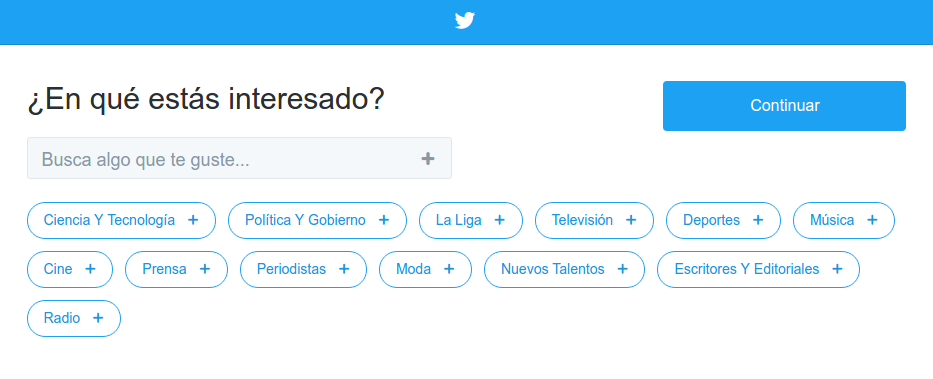
\includegraphics[width=1\textwidth]{./figures/twitter-interest.png}
\caption[Cuestionario de la red social twitter]{Cuestionario de la red social twitter al crear una nueva cuenta (Junio 2016). Fuente: \href{https://www.twitter.com/}{https://www.twitter.com/}}
\label{fig:twitter-interest}
\end{center}
\end{figure}

Cuando las recomendaciones dependen de las opiniones de los usuarios, como en el caso de las técnicas colaborativas, surge otro problema conocido como ``vote early and often'' o votar pronto y a menudo en español. Este fenómeno, consiste en \textbf{manipular} de alguna manera los votos o en este caso las recomendaciones. En el caso de que cualquiera pueda realizar todas las recomendaciones que desee, los creadores de contenido o proveedores de distintos productos o servicios recurrirán a votar en favor de sus elementos y en detrimento de sus competidores.

\subsubsection{Comparación de técnicas}
Existen problemas van ligados a la técnica escogida, y todas las técnicas presentan una serie de ventajas y desventajas entre sí.

Uno de los problemas más conocidos, es el problema del \textit{comienzo frío} (cold start) o cuesta arriba (ramp-up) \cite{lee2001collaborative}. Este problema se puede dar en dos casos, cuando aparece un nuevo usuario\cite{Rashid:2002:GKY:502716.502737} y cuando aparece un nuevo ítem. Cuando aparece un nuevo usuario no se tiene información de él, y en el caso de ser necesario relacionarlo con algún otro usuario o con algún perfil concreto resulta complicado. El caso de un nuevo ítem es similar. Cuando aparece un nuevo ítem y apenas existen recomendaciones sobre este, aparecen problemas a la hora de relacionar este nuevo ítem con otros. En ambos casos, si el sistema requiere de recomendaciones, es necesario que este presente algún tipo de incentivo para que los usuarios realicen valoraciones sobre los elementos.

En el caso de los sistemas \textbf{colaborativos}, estos se ven afectados por los problemas tanto de nuevo usuario como de nuevo ítem, lo cual provoca que estos sistemas no puedan comenzar a funcionar hasta tener información tanto de usuarios como de ítems lo suficientemente amplia como para poder realizar recomendaciones. 

Debido a sus características, este sistema presenta problemas en aquellos entornos en los que existen pocos usuarios y estos evalúan continuamente los mismos ítems. problema conocido como \textbf{dispersión} o problema de la matriz dispersa\cite{Huang:2004:AAR:963770.963775}, o bien los usuarios tienen gustos muy diferentes. En definitiva, este tipo de sistemas resulta útil cuando existe un número suficientemente amplio de usuarios y con una variedad de gustos aceptable dentro del dominio del problema. En \cite{lee2001collaborative}, además del problema clásico del \textit{comienzo frío}, se tratan también estos problemas relativos a la escasa cantidad de recomendaciones.

Debido al enfoque de este tipo de sistemas en los que se depende enormemente de los usuarios, su actitud y predisposición, estos son especialmente sensibles a los problemas que se han analizado en la sección \ref{sec:problemas}. Es especialmente necesario en estos sistemas el incentivar a los usuarios a realizar las valoraciones de los productos, para evitar tanto los problemas del \textit{comienzo frío} como los de la dispersión. También, es en estos sistemas donde existe una mayor problemática con la privacidad, debido a que se utiliza la información de estos en las recomendaciones a otros usuarios desconocidos.

Una de las ventajas que presentan estos sistemas respecto a otros es principalmente su capacidad para poder recomendar elementos que pese a que no estén dentro del mismo grupo, pueden estar relacionados de alguna manera. Por ejemplo, puede darse la situación de que a todos aquellos a los que les gusta la música Jazz les guste también el mismo grupo de Rock, y este sistema sería capaz de recomendar dicho grupo, mientras que otros como por ejemplo el basado en contenido no podría. Otra gran ventaja de esta técnica es la de ser independiente de la representación a nivel de computador de los elementos que recomienda. Debido a esto es frecuentemente usado en la recomendación de elementos u objetos complejos como libros, música, imágenes o elementos multimedia en general.

Los sistemas \textbf{basados en contenido} sufren de manera menor del problema de la dispersión debido a que solo tienen en cuenta las valoraciones del propio usuario y no de todos los usuarios. A pesar de esto, tienen el mismo problema de comienzo en frío que tenían los sistemas colaborativos cuando aparece un nuevo usuario. Es con la aparición de un nuevo ítem con lo que este tipo de sistemas no tiene problema. A pesar de que esta aparición de nuevos elementos no presenta un problema para estos sistemas, lo hace por otra parte el formato que deben presentar estos elementos. Debido a que están fuertemente ligados con las técnicas de filtrado y recuperación de información, presentan el inconveniente de funcionar de manera muy pobre en aquellos escenarios en los que los sistemas a recomendar no se encuentran representados de manera textual. Además, las características y valores de estos elementos deben presentar una estructura común, de manera que puedan consultarse y recuperarse estos atributos de manera automatizada. 

Otro problema que tiene en común con los colaborativos, surge como consecuencia de que estos sistemas generalmente no deben recomendar un objeto que el usuario ya ha valorado, y que por tanto, se entiende que dispone de él o lo conoce lo suficiente. Aunque esta condición no es obligatoria, ya que el puede ser útil recomendar algo que el usuario ya haya seleccionado anteriormente, sí puede no ser deseada. El problema que se presenta aquí es el de distinguir cuando dos elementos son lo suficientemente parecidos para ser considerados iguales y no ser recomendados al mismo usuario cuando este ya ha consumido o valorado uno de ellos.

La sobre especialización es otro problema común. Este tipo de sistemas presentan carencias a la hora de sugerir novedades a los usuarios que les puedan interesar, y además presentan dificultades a la hora de adaptarse a los cambios de gustos o intereses de los usuarios. Es necesario pues, que en algunos casos, se establezcan mecanismos que se encarguen de introducir este factor de aleatoriedad, de manera que se sugieran nuevos elementos para así ampliar el abanico de gustos e intereses del usuario sin estancarse en un solo campo.

Los sistemas \textbf{demográficos} también sufren el problema del \textit{comienzo frío}, pero solo respecto a la aparición de nuevos ítems. También comparten otro de los problemas de los colaborativos que es el de identificar a usuarios que se salen de lo común, es decir, que o bien no tienen características en común con ninguno de los actuales grupos, o presentan algunas características de cada grupo, pero no las suficientes como para categorizarlos en uno concreto. Pese a no tener el problema de \textit{comienzo frío} con los nuevos usuarios, necesitan recopilar información sobre los distintos perfiles antes de comenzar a operar. Esta recopilación y formación de perfiles es su principal diferencia respecto a los sistemas colaborativos.

Pese a que estos sistemas mencionados anteriormente, que están basados en el aprendizaje durante la ejecución, parecen tener muchos problemas especialmente al inició, presentan la ventaja de ser más flexibles y adaptativos que las dos técnicas que se verán a continuación. Tanto los sistemas basados en utilidad como los basados en conocimiento carecen de los problemas de \textit{comienzo frío} y de dispersión ya que no aprenden durante su ejecución. Sin embargo, en ambos casos es necesario un gran trabajo previo.

En el caso de los sistemas \textbf{basados en utilidad}, pese a carecer del problema del \textit{comienzo frío}, necesitan crear la función de utilidad considerando todas las características del objeto. Esto supone un gran trabajo al inicio y mucha interacción con el usuario, lo cual supone una desventaja para usuarios inexpertos o usuarios que no quieren invertir demasiado tiempo en esto, pero que facilita en gran medida el filtro y selección de aquellos usuarios expertos o que buscan elementos con unas características muy específicas. Como se mencionó en la sección anterior, la gran ventaja de estos sistemas es poder considerar aquellas propiedades que no son intrínsecas al objeto, como el tiempo o el formato del envío. Esto los hace especialmente útiles en sistemas de comercio online.

Por otra parte, los sistemas \textbf{basados en conocimiento} comparten el problema de la recolección de datos o conocimiento con los sistemas clásicos basados en el conocimiento, en los que se necesita de un experto del que extraer información y de un ingeniero del conocimiento que sea capaz de extraer dicha información. Respecto a los tipos de conocimiento que estos sistemas requieren se pueden categorizar en tres. Por una parte encontramos el conocimiento sobre los ítems o elementos que se van a recomendar. También encontramos el conocimiento sobre el usuario y las necesidades de este. Finalmente está el conocimiento funcional, que permite establecer relación entre las necesidades del usuario y las características de los objetos.
%En general no se si tengo suficientes citas, ya que solo he puesto las que me he leído, no se si en alguna parte o en algun caso sería recomendable poner alguna más que tu consideres

\subsection{Sistemas de recomendación híbridos}
\label{sec:sistemas-hibridos}

En la sección anterior se ha visto que cada tipo de sistema de recomendación tiene unas fortalezas y debilidades, las cuales, en muchos casos, son complementarias. Es decir, algunas técnicas proveen de aquello que les falta a otras y viceversa. Siendo esto así, surge una idea, la de combinar varios de estas técnicas, tratando de buscar sacar el máximo potencial posible de cada una. En general la mayoría de estos sistemas tratan de solventar los problemas de los sistemas colaborativos del nuevo usuario y el nuevo item combinándolo con alguna otra técnica.

Existen varios mecanismos a la hora de combinar las técnicas vistas anteriormente. Estos mecanismos permiten combinar no solo dos de las técnicas anteriores, sino tantas como se desee. Además, algunos de estos mecanismos permiten combinar las salidas de otros entre sí o con otras técnicas de recomendación, ofreciendo de esta manera gran posibilidad de personalización y adaptación al problema en cuestión. En \cite{burke2007hybrid} se realiza un análisis de sistemas que emplean algunas de estrategias de hibridación, comparando estos sistemas y analizando que tipo de técnicas funcionan mejor según que estrategias o métodos se empleen de los que se muestran a continuación.

A continuación se muestran los mecanismos disponibles:

\subsubsection{Ponderado}
Los sistemas ponderados son aquellos en los que la utilidad o puntuación de un determinado elemento para un usuario, es calculado a partir de la puntuación proporcionada por las diferentes técnicas utilizadas. Se pueden usar diferentes aproximaciones a la hora de combinar estas puntuaciones, desde una simple media ponderada que puede ir variando conforme varíen la información disponible, a sistemas de consenso\cite{Pazzani:1999:FCC:340120.340130}.

\subsubsection{Conmutado}
En un sistema conmutado se alterna entre diferentes técnicas de recomendación dependiendo de alguna condición \cite{tran2000hybrid}. De esta manera, puede usarse un sistema basado en contenido mientras no existan suficientes valoraciones para relacionar usuarios, y más adelante, conforme se comiencen a recoger más y más valoraciones pasar a utilizar técnicas colaborativas. También puede emplearse para recurrir a otra técnica cuando la primera falle o no genere un resultado lo suficientemente bueno.

\subsubsection{Combinado}
Este tipo de sistema, combina las recomendaciones proporcionadas por varios tipos de técnicas, y se las ofrece al usuario\cite{Cotter:2000:PIP:647288.760209}. De esta manera, se pueden utilizar varias técnicas que usen información diferente, de manera que se superen problemas como el del estancamiento o sobre especialización que traen consigo los sistemas basados en contenido y problemas por ejemplo de nuevo item de los sistemas colaborativos.

\subsubsection{Combinación de características}
Este tipo de mecanismo busca combinar las características de varios tipos de técnicas en una sola. Por ejemplo, se puede enriquecer la información de los sistemas basados en contenido a partir de las relaciones existentes entre los usuarios que han valorado dichos elementos, las cuales son extrapoladas de la aplicación de las técnicas colaborativas o demográficas.

\subsubsection{Cascada}
En los sistemas que emplean este tipo de mecanismos, se realizan filtros progresivos en los que se van seleccionando y filtrando mediante varias técnicas aquellos elementos que se recomendarán al usuario. La recomendación se realiza mediante etapas, donde cada técnica realiza una selección del conjunto de elementos que le proporciona la anterior, o en caso de ser la primera de todo el conjunto disponible. Esto puede servir para liberar de carga computacional a aquellas técnicas que sean más costosas, utilizando un primer filtro que elimine aquellos elementos que con total seguridad no van a ser deseados por el usuario.

\subsubsection{Aumento de las características}
La salida proporcionada por la aplicación de alguna técnica de recomendación se convierte en la entrada de otra en este tipo de sistemas\cite{Sarwar:1998:UFA:289444.289509}. De esta manera, la valoración producida por una técnica se incorpora al proceso de recomendación de la segunda. Difiere del mecanismo en cascada en que esta técnica de cascada no usa las salidas producidas por estas en su valoración, sino que simplemente la segunda técnica opera sobre aquellos elementos que han pasado el primer filtro, sin tener ningún conocimiento del proceso seguido ni de lo que existía anteriormente. Tampoco se tiene acceso en el mecanismo de cascada a la valoración proporcionada por el mecanismo anterior.

\subsubsection{Meta-nivel}
En este tipo de sistemas\cite{Balabanovic:1997:FCC:245108.245124}, lo que se pasa como entrada a la siguiente técnica es el modelo generado por la primera, y no la salida como ocurría en el método de aumento de las características. Es especialmente útil para que el segundo método trabaje con información más compacta que si trabajase sobre el total de la información, evitando de esta manera el problema de trabajar con gran cantidad de datos. Además, al trabajar con información más compacta también se reduce el problema de la matriz dispersa que se mencionaba anteriormente, ya que en el modelo que se pasa como resultado, se eliminan muchas dimensiones y se presentan modelos que agrupan diversas valoraciones de elementos.



% Local Variables:
%  coding: utf-8
%  mode: latex
%  mode: flyspell
%  ispell-local-dictionary: "castellano8"
% End:
